% !TEX root = ../NeuralNetworksEN.tex


%%%%%%%%%%%%%%%%%%%%%%%%%%%%%%%%%%%%%%%%%%%%%%%%%%%%%%%%%%

\section{Generative neural networks}

Instead of using neural networks to analyze images, the paper~\cite{goodfellow2014generative} has shown in 2014 that they can be used \guill{backwards} to generate images.
%
These generative neural networks, for example, find applications for special effects, video games and artistic creation.
%
Similar questions and methods can be found in the training of autonomous cars and to solve strategy games.
%
Figure~\ref{fig:generative} shows the structure of such a network $g_{\mygreen{w}}$, which depends on weights $\mygreen{w}$. The layers somehow play mirror roles compared to the architecture of the discriminating neural networks exposed in the previous article.
%
From an entry ${\color{red} y}$ composed of a small number of values, which are typically drawn randomly, one generates an image ${\color{blue} x} = g_{\mygreen{ w}}({\color{red} y})$.

\begin{figure}\centering
	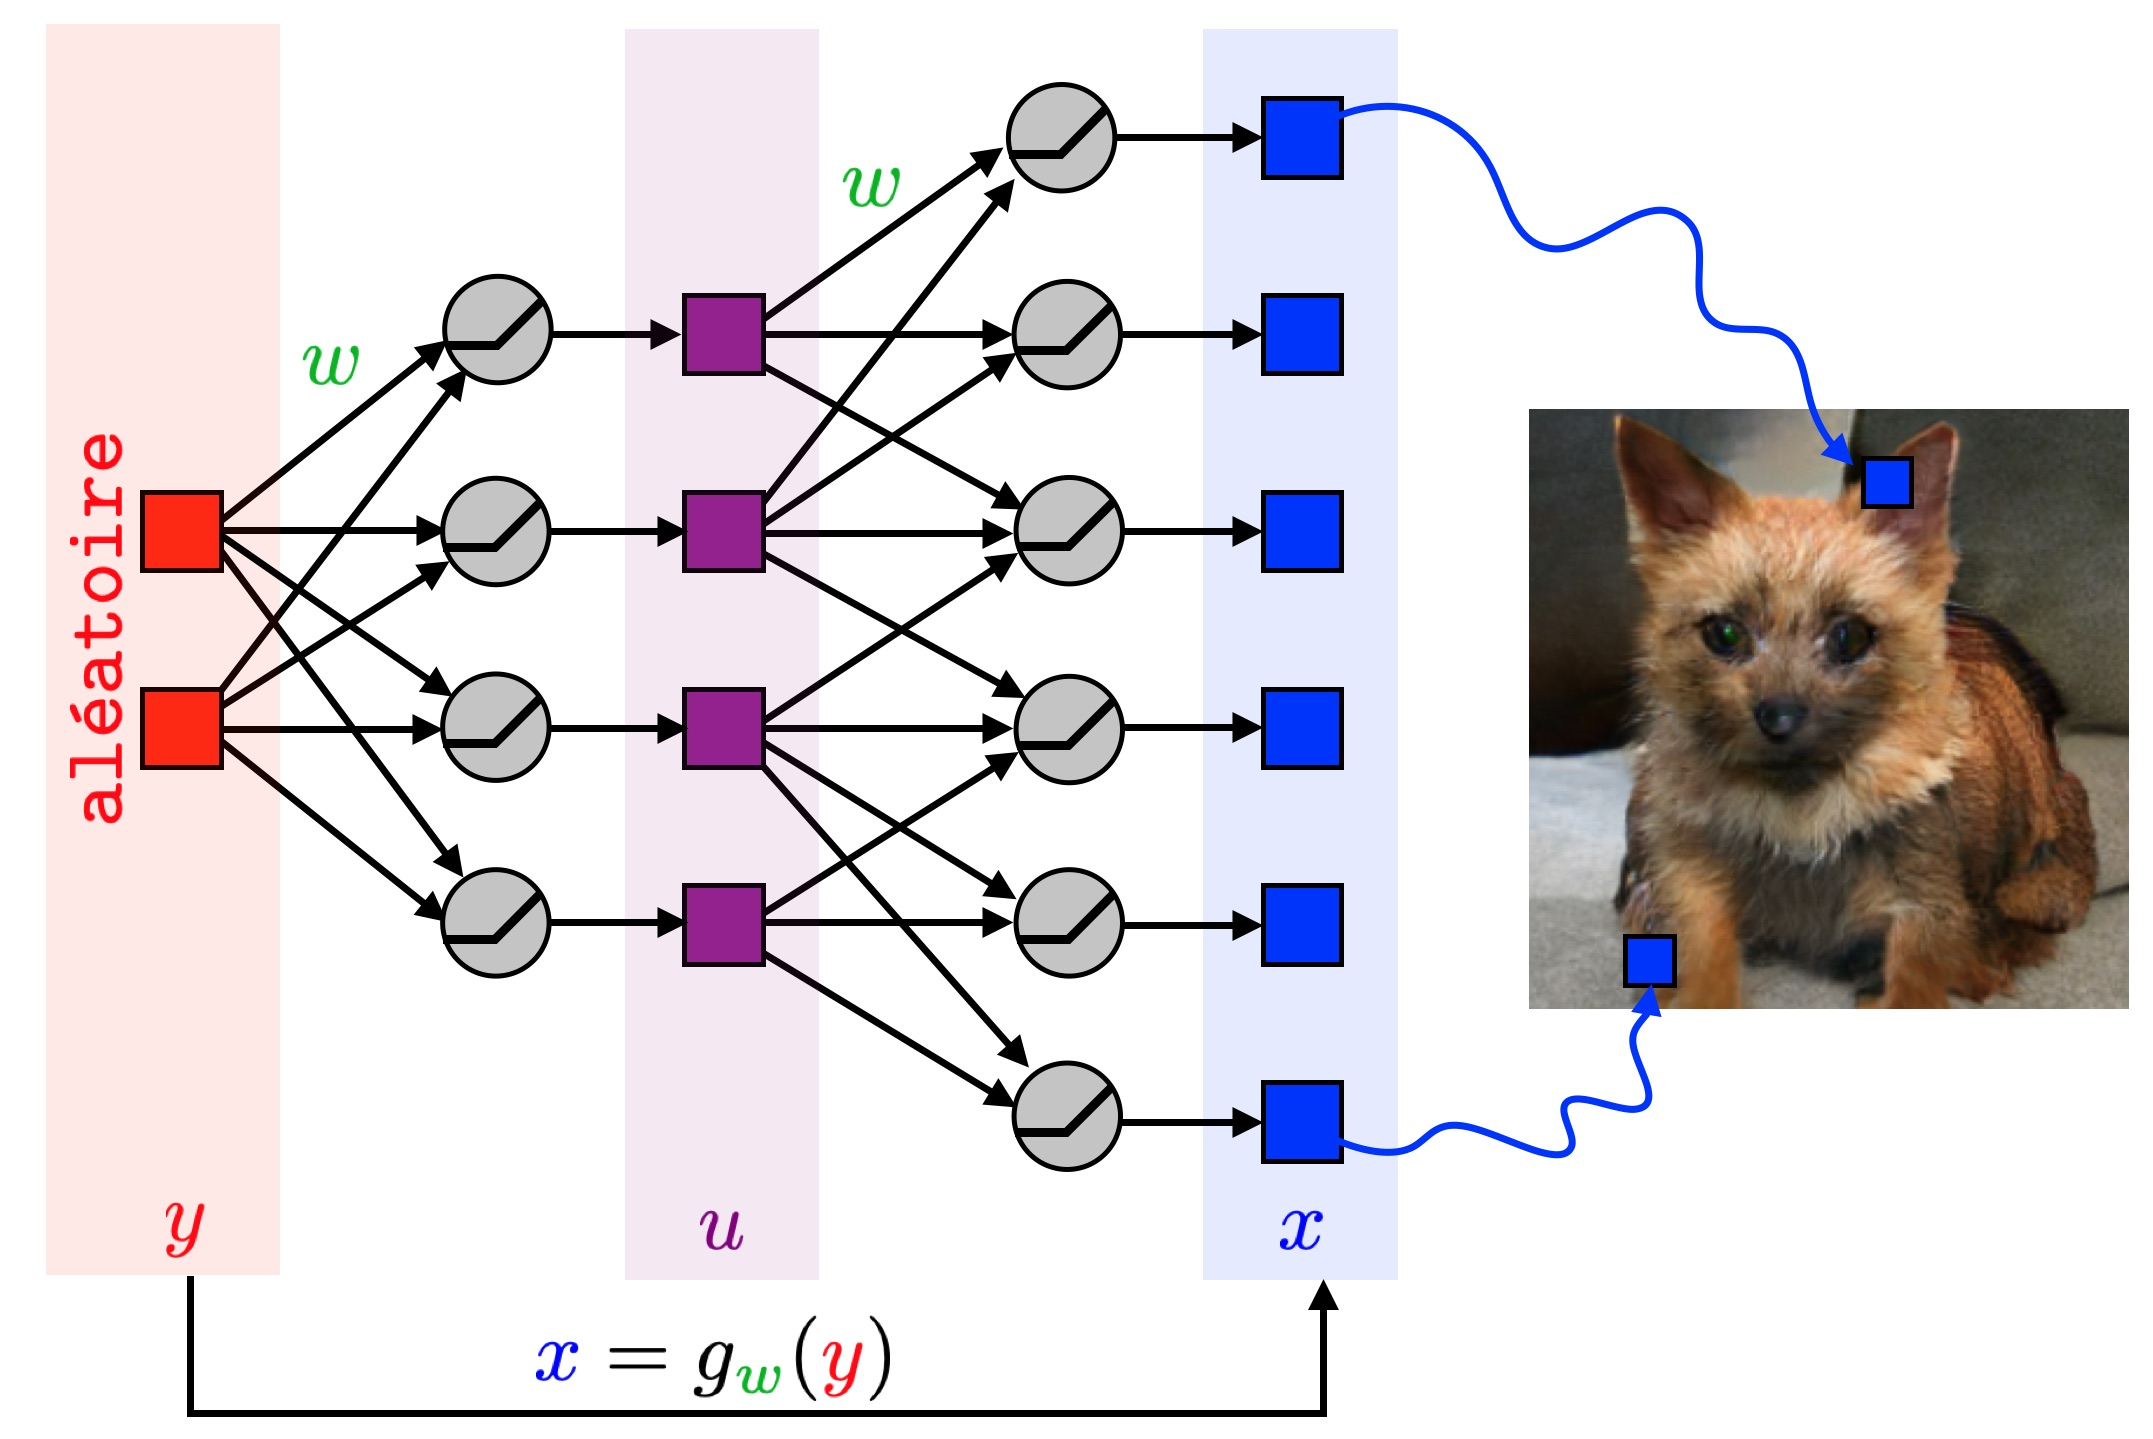
\includegraphics[width=.8\linewidth]{generative}
\caption{\label{fig:generative} Example of a simplified generative neural network (a network for generating such complex images has more layers).  }
\end{figure}

The problem of training such networks is unsupervised: there is only a large number of training images, without indication of what they contain.
%
There is no longer any need for human intervention to indicate to the network the content of the images which it must recognize.
Data collection is thus simpler than for training discriminatory networks. In addition, this principle of unsupervised learning is close to the way children learn, mainly by observing and manipulating the world around them.
%
The goal is then to select the weights $\mygreen{w}$ of the neurons of the network $g_\mygreen{w}$ so that the random images generated (the \guill{fake} images) resemble as closely as possible the images of the training set.

%%%%%%%%%%%%%%%%%%%%%%%%%%%%%%%%%%%%%%%%%%%%%%%%%%%%%%%%%%
\section{Unsupervised learning of generative networks}
\label{sec-app-gen}

The goal of generative neural networks is not to solve a task such as recognizing objects in images.
%
In order to train the weights $\mygreen{w}$ of the network, the problem must be formalized mathematically. This involves generating a set of \guill{virtual} images (the false ones) that look like real images in a database. It is not simply that a generated image looks like a real image, it is necessary to match the two sets of images. For example, if in the database there are half images of dogs and half images of cats, the network must also generate half of dogs and half of cats.

We will write $\{\mylblue{z_1, z_2, \ldots, z_n}\}$ the set of $n$ images in the database. The number $n$ of images is very large, of the order of several thousand or millions. Given a generative neural network $g_{\mygreen{w}}$, which is parameterized by its weights $\mygreen{w}$, we note $\{\myblue{x_1, x_2, \ldots, x_n} \}$ a set of $n$ \guill{false} images randomly generated by the network. To generate the first false image $\mylblue{x_1}$, this means that we randomly draw the input values ${\color{red} y_1}$ and apply the network to these inputs, to obtain the virtual image $\mylblue{x_1} = g_{\mygreen{w}}({\color{red} y_1})$. We then do the same thing with $\mylblue{x_2} = g_{\mygreen{w}} ({\color{red} y_2})$ and so on.

The goal of unsupervised learning is therefore to find weights $\mygreen{w}$ so that the set of false images $\{\myblue{x_1, \ldots, x_n} \}$ is as close as possible to the set of images $\{\mylblue{z_1, \ldots, z_n}\}$ of the database. The optimization problem is written thus
\eq{
	\umin{\mygreen{w}} \text{Distance}( 
		\{\myblue{x_1,\ldots,x_n} \}, 
		\{\mylblue{z_1,\ldots,z_n}\}  ).
}
It should here be remembered that the images generated $\{\myblue{x_1, \ldots, x_n} \}$ depend on the network $g_{\mygreen{w}}$ and therefore on the weights $\mygreen{w}$. We can reformulate the previous problem as
\eq{
	\umin{\mygreen{w}} \text{Distance}( 
		\{g_{\mygreen{w}}({\color{red}y_1}),\ldots, g_{\mygreen{w}}({\color{red}y_n})\}, 
		\{\mylblue{z_1,\ldots,z_n}\}  ).
}
%
The mathematical question that arises is therefore to define a notion of distance between two sets of points. There are many ways to do this, and we will explain one that is well suited to this learning problem.
%
It exploits the theory of optimal transport.


%%%%%%%%%%%%%%%%%%%%%%%%%%%%%%%%%%%%%%%%%%%%%%%%%%%%%%%%%%
\section{Monge's optimal transport}
\label{sec-ot}

The optimal transport problem is formulated by Gaspard Monge~\cite{Monge1781} in 1781, for military applications.
%
The question asked is to determine the most economical way to transfer objects from a set of sources $\{\myblue{x_1, \ldots, x_n}\}$ to a set of destinations $\{\mylblue{z_1, \ldots, z_n}\}$. For Monge, it is a matter of transferring soil from cuttings to create embankments. But this question finds a multitude of applications.
%
For the problem of training generative networks, the sources are the false images generated by the network and the destinations are the images of the database.

\newcommand{\perm}[1]{s_{#1}}

It is thus necessary to link each source, for example $\myblue{x_1}$ to a single destination point, which we will note $\mylblue{z_{\perm{1}}}$, where $\perm{1}$ is an integer between $1$ and $n$. Similarly, ${\color{blue} x_2}$ is linked to $\mylblue{z_{\perm{2}}}$ and so on. For example, in figure~\ref{fig:otmonge}, we link $\myblue{x_2}$ to $\mylblue{z_5}$, which means that $\perm{\myblue{2}} = \mylblue{5}$.
%
Each of the $n$ destinations must also be supplied by a source. This means for example that ${\color{blue} x_1}$ and ${\color{blue} x_2}$ cannot be linked to the same destination, all the sources must be linked to different destinations. This means that $\{\perm{1}, \ldots, \perm{n}\}$ must be a permutation of the first $n$ integer numbers.
%
For example, on the figure~\ref{fig:otmonge}, on a simple example with $n=6$ elements, we have chosen on the left the permutation
\eq{
	(\perm{\myblue{1}}=\mylblue{1},
	\perm{\myblue{2}}=\mylblue{5},
	\perm{\myblue{3}}=\mylblue{4},
	\perm{\myblue{4}}=\mylblue{6},
	\perm{\myblue{5}}=\mylblue{3},
	\perm{\myblue{6}}=\mylblue{2}).
}
%
Monge's problem then consists in finding the permutation which minimizes the sum of the transport costs. Monge decided that the cost of transportation between a source $\myblue{x}$ and a destination $\mylblue{z}$ is equal to the Euclidean distance $\norm {\myblue{x} - \mylblue{z}}$ between the two points, but one can choose another cost: for example a travelling time or the price required for gasoline if using trucks, etc. We have to solve the problem
\eq{
	\umin{\text{permutation } s} 
		\norm{\myblue{x_1} - \mylblue{z_{\perm{1}}}} + 
		\norm{\myblue{x_2} - \mylblue{z_{\perm{2}}}} + 
		\ldots + 
		\norm{\myblue{x_n} - \mylblue{z_{\perm{n}}}}.
}
Once we have calculated an optimal permutation $s^\star = (\perm{1}^\star, \ldots, \perm{n}^\star)$ (i.e. which is solution of the previous problem), we define the distance between the sets of points as the value of the total transport cost
\eq{
	\text{Distance}( 
		\{\myblue{x_1,\ldots,x_n} \}, 
		\{\mylblue{z_1,\ldots,z_n}\}  ) 
	\eqdef 
		\norm{\myblue{x_1} - \mylblue{z_{\perm{1}^\star}}} + 
		\norm{\myblue{x_2} - \mylblue{z_{\perm{2}^\star}}} + 
		\ldots + 
		\norm{\myblue{x_n} - \mylblue{z_{\perm{n}^\star}}}.
}

\begin{figure}\centering
	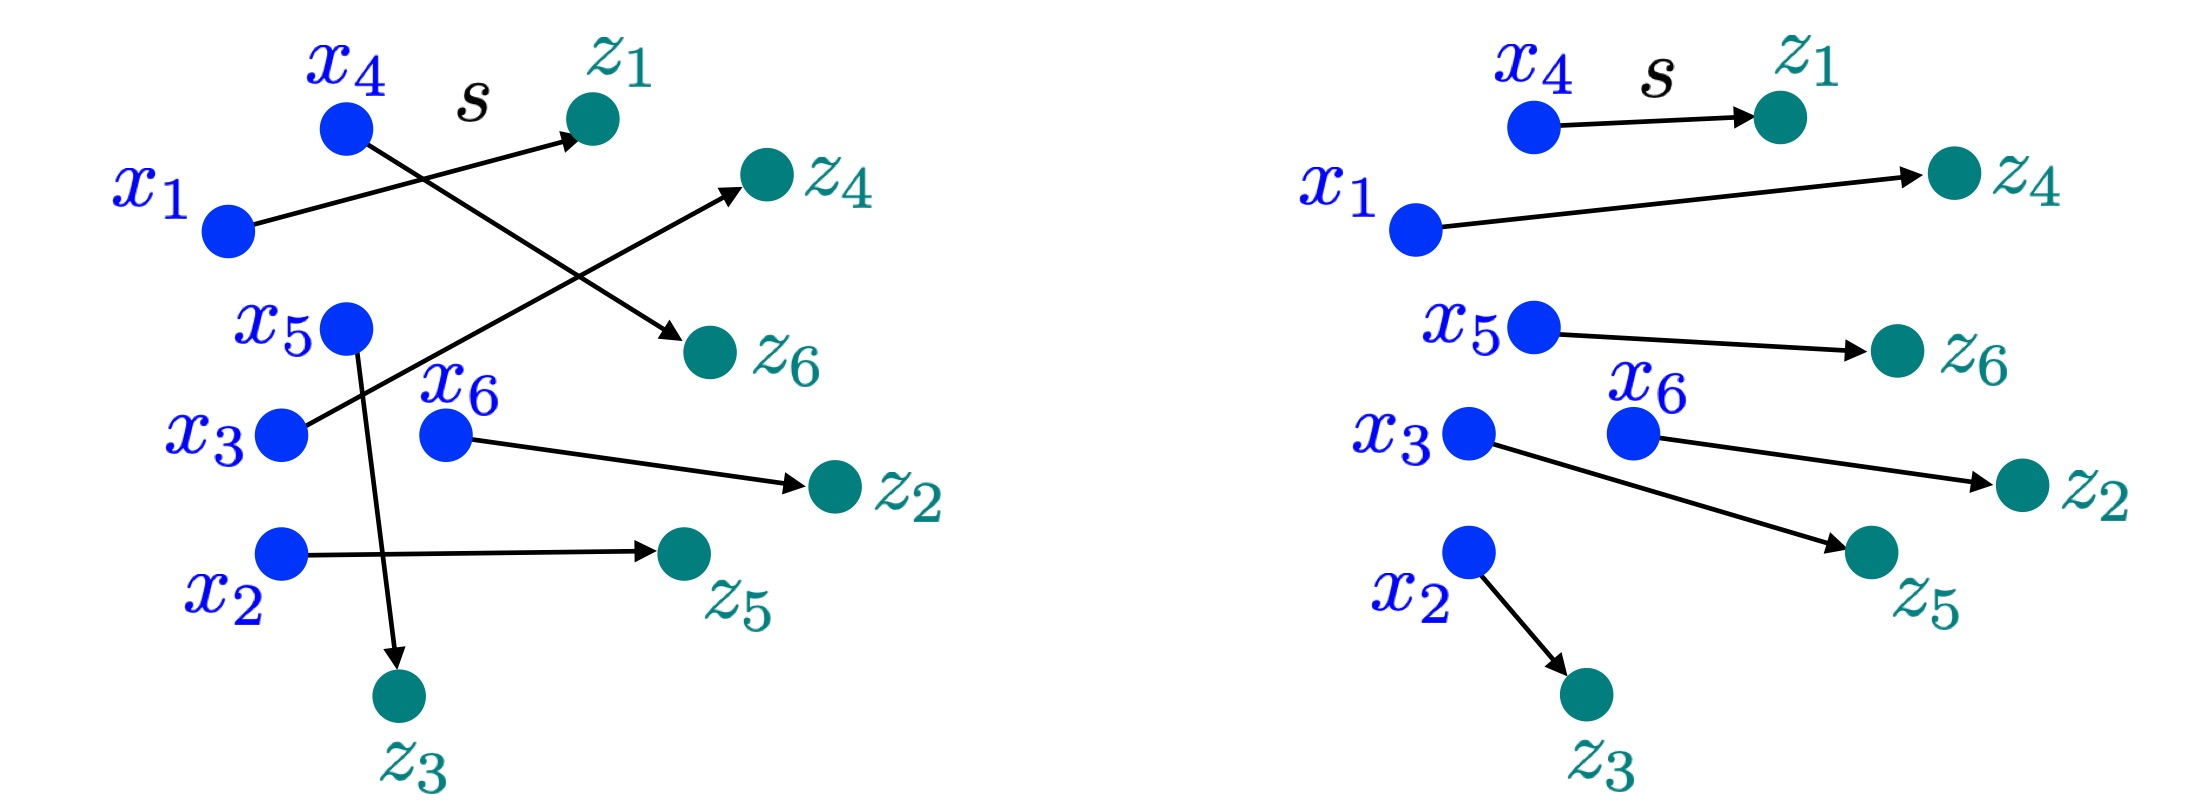
\includegraphics[width=.8\linewidth]{otmonge.jpg}
\caption{\label{fig:otmonge} Example on the left of a non-optimal permutation $s$ and on the right of the optimal permutation, in the case of $6$ points in dimension 2.  }
\end{figure}

The difficulty in calculating this distance is that the total number of permutations to be tested is very large. Indeed, for the choice of $\perm{1}$ there are $n$ possibilities, for that of $\perm{2}$ there is $n-1$ (since the value of $\perm{1}$ is taken), for $\perm{2}$ there is $n-2$, etc. So the total number of permutations is $n!$, The factorial of the number $n$, which is defined as
\eq{
	n! = n \times (n-1) \times (n-2) \times \ldots \times 2 \times 1.
}
For $n=6$ as in the figure~\ref{fig:otmonge}, there is therefore
\eq{
	6! = 6 \times 5 \times 4 \times 3 \times 2 \times 1 = 720 \text{ possible permutations.}
}
In this simple case, we can test them all and choose the best one, which is, as shown on the right of the figure~\ref{fig:otmonge},
\eq{
	(\perm{\myblue{1}}=\mylblue{4},
	\perm{\myblue{2}}=\mylblue{3},
	\perm{\myblue{3}}=\mylblue{5},
	\perm{\myblue{4}}=\mylblue{1},
	\perm{\myblue{5}}=\mylblue{6},
	\perm{\myblue{6}}=\mylblue{2}).
}
The difficulty is that for $n = 70$, there are more than $10^{100}$ possibilities, which is to be compared to the $10^{79}$ atoms in the universe \ldots And to train neural networks, $n$ is even much bigger!
%
It was therefore necessary to wait for several mathematical and algorithmic revolutions before being able to obtain a method enabling this problem to be resolved.


%%%%%%%%%%%%%%%%%%%%%%%%%%%%%%%%%%%%%%%%%%%%%%%%%%%%%%%%%%
\section{The optimal transport of Kantorovitch}
\label{sec-kanto}

Monge has noticed that the solutions to his problem have very specific structures. For example, we can observe in the figure~\ref{fig:otmonge}, on the right, that the optimal paths do not cross, and Monge proved it in his article~\cite{Monge1781}. But this is not enough to solve the problem, because there are still a lot of paths without crossing. It took over 200 years to figure out how to get more information about the solutions in order to calculate them efficiently.
%
It was Leonid Kantorovitch who found, in 1942~\cite{Kantorovich42}, a new formulation of the problem of optimal transport. He allowed each source to be divided into several parts, for example two equal parts with a weighting of 1/2 each. This division of production is interesting because it simplifies the optimization problem. It is also natural for the problem studied by Kantorovitch who was trying to model and plan production in economics. He won the Nobel Prize in economics for this idea.
%
Together with these pioneering works by Kantorovitch, George Dantzig introduced in 1947 the simplex algorithm~\cite{dantzig1990origins}, which makes it possible to efficiently solve large scale transport problems. Its numerical complexity to solve an optimal transport problem between $n$ points is of the order of $n^3 = n \times n \times n$, which is much lower than $n! = n  \times (n-1) \times \ldots \times 2 \times 1$. It is at the heart of a very large number of industrial systems which must optimize the adequacy between means of production and consumption. And we can also use it to train generative neural networks! One can look at~\cite{PeyreCuturi} for more details on the optimal transport theory, efficient algorithms and its applications to data science.


%%%%%%%%%%%%%%%%%%%%%%%%%%%%%%%%%%%%%%%%%%%%%%%%%%%%%%%%%%
\section{Adversarial networks}

One difficulty in applying optimal transport to generate generative networks is that it is necessary to choose the transport cost between two images.
%
We could calculate the Euclidean distance between the pixels of the images, but this does not work well, because it does not take into account the geometry of the objects present in the images.
%
A very successful idea was introduced in 2014 by Ian Goodfellow and his collaborators~\cite{goodfellow2014generative}. It can be interpreted as using a second neural network to determine this transport cost~\cite{martin2017wasserstein}.
%
This second network $f$, called adversary network, plays a discriminative role. While the goal of the generator $g$ is to generate  fake images which looks real, the goal of $f$ is, on the contrary, to do its best to recognize true and false images. These two networks are jointly trained, this is why one speaks of adversarial networks.
%
The training of these two networks corresponds to what is called a zero-sum game, introduced by John Von Neumann in 1944~\cite{morgenstern1953theory} and then generalized by John Nash in 1950~\cite{nash1950equilibrium}, which just like Kantorovitch obtained the Nobel Prize in economics.

These recent advances~\cite{goodfellow2014generative} have made it possible to obtain excellent results for image generation.
%
The figure~\ref{fig:deepfake} shows results obtained with the method explained in~\cite{brock2018large} and its use to calculate \guill{paths} of images between dogs and cats.

\begin{figure}\centering
	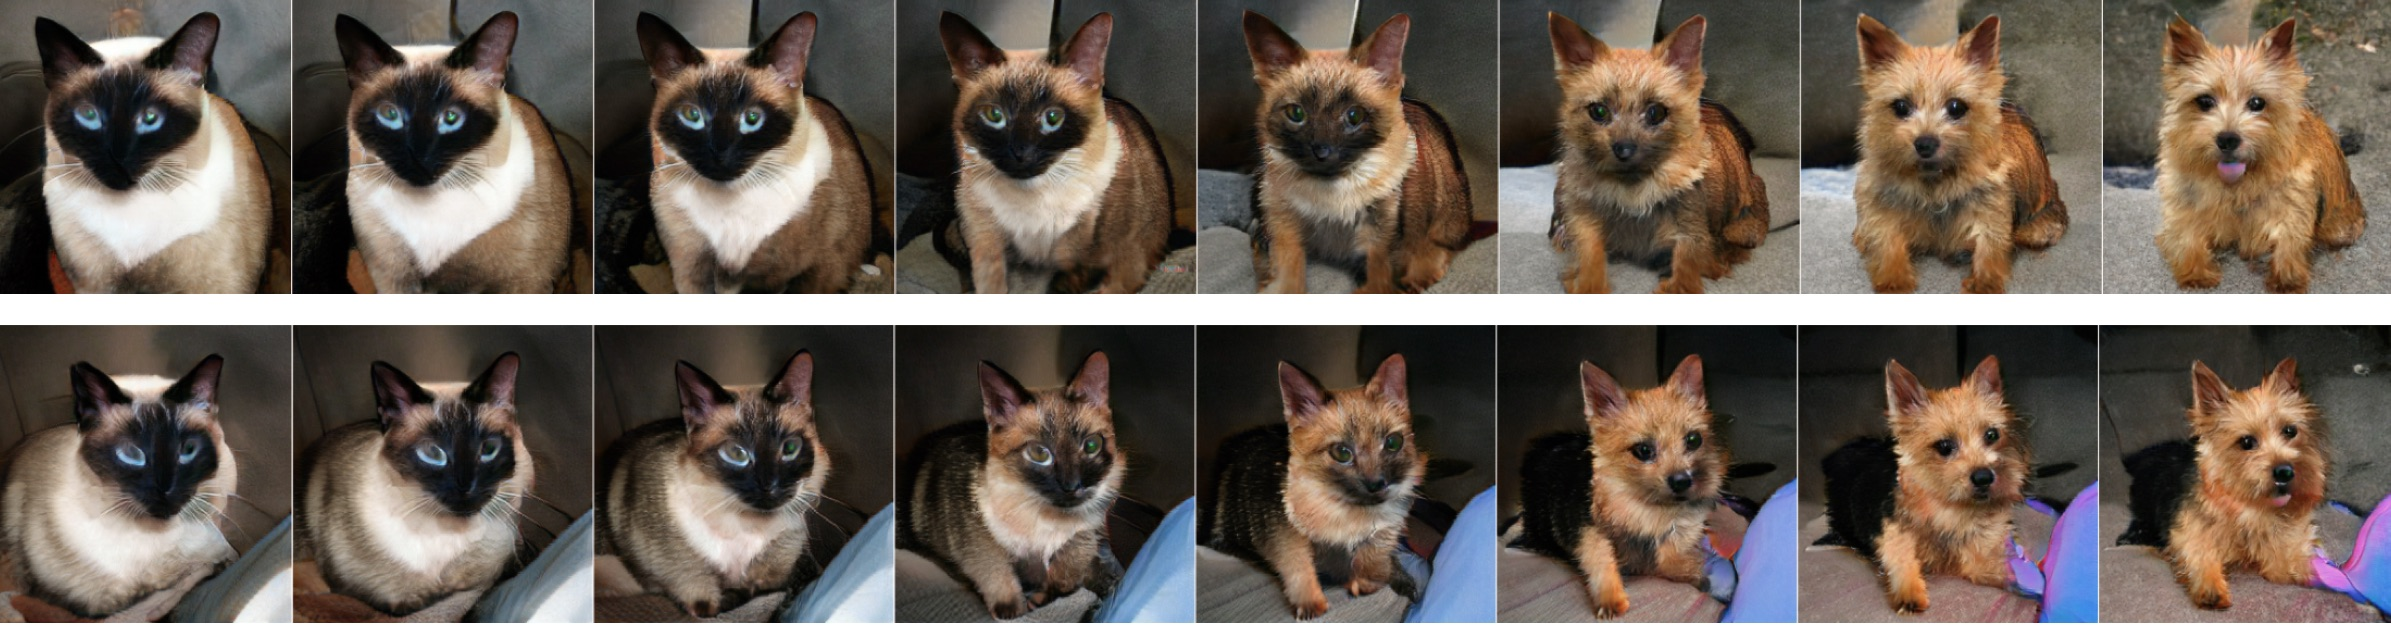
\includegraphics[width=.95\linewidth]{deepfake}
\caption{\label{fig:deepfake} Two examples of \guill{deep fakes} which are virtual images interpolating between cats and dogs. }
\end{figure}


